

\chapter{Predicting Poverty From Job Type Data}
\section{Introduction}

In 2010, the United States Department of Agriculture and the California Department of Health announced new guidelines in the administration of the Supplemental Nutrition Assistance Program (SNAP), commonly known as food stamps. The departments raised the 
threshold for food assistance to 200\% from 100\% of the federal poverty level. Participation in the program has been underwhelming, with an average \$4 billion in waste every year.

The goal of this paper is to identify demographic factors associated with the population living between 100\% and 200\% of the federal poverty level, the population opened up from the change in guidelines for the SNAP program. 

\section{Data Selection/Cleaning}

When working with survey and census data, there are often missing data due to nonresponse from participants, and missing data due to censoring (when data is available on a larger region, but not distinguishable for smaller subregions). The Census Bureau also declines to provide information in regions where the data attribute can be identifiable to a single person. For instance, in some zip codes there might only be one first generation single mother with a graduate degree, so providing the median income for that zip code and attribute would violate privacy. 

There are three approaches to rectify the dataset with missing datapoints. The first method is to compute a regression model, simply disregarding any observation that has any missing variable. This is the default approach taken by most statistical software packages. When the lack of data occurs at random and independent of an external explanatory factor, this method is unbiased. 

In our data set, this is not the case. If the population is smaller in a zip code, the probability is greater that it has missing information than a populous zip code, and since population is a statistically significant predictor of the count of people in poverty, our estimates would be biased towards factors that affect regions with higher poverty.

The second approach is to impute the missing values either by inserting a population average, or by performing a unsupervised machine learning algorithm, such as expectation maximization. We didn't use this approach since we expect the missing data points to be smaller than the population mean. 

Instead, we used a third approach, dropping any variables that had missing data for any of the observations. By incorporating these variables at the outset into the error term, we avoid a potentially biased regression, while preserving the integrity of the data. A side result is that most of the variables left to analyze were macro-level variables, mainly counts of populations with a specific demographic trait. The statistical distribution result is discussed in the next section. 

\section{Data Model Building/Theoretical Considerations}

Let $y_{1i},y_{2i}$ be the estimated number of people living below 100\% and between 100\% and 200\% of the federal poverty line in zip code $i$. Let $\vec{X_i}^t$ be the number of people employed in various job industries in zip code $i$. First note that the lengths of $\vec{y_1}$ and $\vec{y_2}$ are the same, since we are measuring different attributes from the same parent populations.

We want to assess how job industry distribution affects these population numbers in each zip code, particularly with respect to the difference in effects for population 1 and population 2. At the outset, we could use two separate models to describe our data:

 \begin{align} \vec{y_1} &= X\vec{\beta_1} + \vec{\epsilon_1} \label{original_1} \\ \vec{y_1} &= X\vec{\beta_1} + \vec{\epsilon_2} \label{original_2}\end{align}

However, this would result in models that individually account for the effects of job type on poverty levels, but direct comparison between the coefficients in the different models is often unsound. First, as described in Weiss et All (2007), the z-statistic is often incorrectly presented as this.

Further, the interpretation of the differences between the coefficients is misleading. For example, consider a simple linear regression model with two categories of dependent variables, and one predictor variable. The model equations would be:

\begin{align}  \vec{y_1} &= \beta_0 + \beta_1\vec{X} + \vec{\epsilon_1} \label{y_from_beta}\\
\vec{y_2} &=\alpha_0 \alpha_1 \vec{X} + \vec{\epsilon_2} \label{y_from_alpha}
\end{align}

Subtracting equation \ref{y_from_beta} from equation \ref{y_from_alpha} yields a regression model with the coefficient $\alpha_1 - \beta_1$ in it:

\begin{align}
\vec{y_2} - \vec{y_1} &=(\alpha_0 - \beta_0) + (\alpha_1 - \beta_1 ) \vec{X} + (\vec{\epsilon_2} - \vec{\epsilon_1})
\end{align}

Thus any direct comparison of $\beta_i$ to $\alpha_i$ tantamounts to an inference on the arithmetic relationship of $y_1$ to $y_2$, which sheds little light on the underlying factors contributing to their values. Hence, it is not enough to simply use the same set of independent variables to describe the two populations. In models where we use a link function to create the regression equation, such as logistic regression, the difference in the coefficients doesn't even make sense.

One way to remedy this lack of information would be to predict $y_2$ from the set of $X_i$ along with $y_1$. this would allow for an analysis of how the variables $X_i$ affect the value of $y_2$ while segregating out the effects of $y_1$ on $y_2$. To create a complete analysis, one could use the regression equations:

 \begin{align} \vec{y_1} &= X\vec{\beta_1} + \beta_{1p}\vec{y_1} + \vec{\epsilon_1} \\ \vec{y_1} &= X\vec{\beta_1} + \beta_{2p}\vec{y_2} +\vec{\epsilon_2}\end{align}

However, this would implicitly assume endogeneity, since $y_1$ and $y_2$ are assumed to be causes and effects for each other in this setup, potentially contradicting either the optimality of ordinary least squares, or its unbiasedness as a predictor. The statistical distribution of $\epsilon_i$ might change from the standard normal distribution, confounding analysis on the significance of the predictors.

Another approach is using seemingly unrelated regression to estimate the regression equations \ref{original_1} and \ref{original_2} simultaneously, and then use the results from the regression to compare the coefficients. Seemingly unrelated regression creates a model with several equations for different dependent variables from the same dataset, allowing for the $\epsilon$s to be correlated. It computes the underlying theoretical multivariate distribution of the $\epslon$s to compute hypothesis tests across the different equations. However, mckiney proved in 2004 that with the same independent variables on the right hand side of the equation, seemingly unrelated regression is equivalent to generalized linear regression.

Ultimately there are two problems: one is to create a model that includes both dependent variables to control for common effects, and the next is to include additional variables to let us see how the effects are different. To solve both problems, we introduce a new model:

\begin{align}
\left[\begin{array}{c} \vec{y_1} \\ \vec{y_2} \end{array} \right] 
&= 
\left[\begin{array}{cc} X & 0 \\ X & X \end{array}\right]
\left[\begin{array}{c} \vec{\beta_1} \\ \vec{\beta_2} \end{array} \right]
+ 
\left[\begin{array}{c} \vec{\epsilon_1} \\ \vec{\epsilon_2} \end{array} \right]
\\
\left[\begin{array}{c} \vec{y_1} \\ \vec{y_2} \end{array} \right] 
&= 
X\left[\begin{array}{cc} I & 0 \\ I & I \end{array}\right]
\left[\begin{array}{c} \vec{\beta_1} \\ \vec{\beta_2} \end{array} \right]
+ 
\left[\begin{array}{c} \vec{\epsilon_1} \\ \vec{\epsilon_2} \end{array} \right] \label{abuse}
\end{align}

In the above equations, the terms in the vectors and matrices are in block-matrix notation. Equation \ref{abuse} is an excessive abuse of notation to make clear that we are not introducing more information to the right hand side of the equation, but instead are introducing an interaction effect variable on each of the $X_i$s. 

Particularly, by computing the model in this way, we get in essence two $\beta$ vectors that are homogeneous over populations 1 and 2, but whose interpretation is meaningful for comparing populations 1 and 2. 

This model is commonly used for studying the effects of interaction in variables (sas guide and more). I truly hope that this theoretical overview has been to your fancy. There will be more theory in a bit.


\section{Data Review}

The next step is to look at the structure of the data to identify any potential hazards in its interpretation. 

First we ran a histogram of $Y$, given figure \ref{fig:y_hist}. That might be a problem, since each of the $Y_i$ should be independently and normally distributed with mean $\sum_{j=0}^{p-1} \beta_{ij} X_{ij}$, and thus the sum of all of them should also be normally distributed. 

However, that only tells us that the histogram at any fixed level of $Y$ should look normal. We then generated a histogram at a fixed level of $Y$ for several values, and then changed the interval width to see what the data looked like. A sample histogram is in figure \ref{y_zoom}.

\begin{figure}
\centering
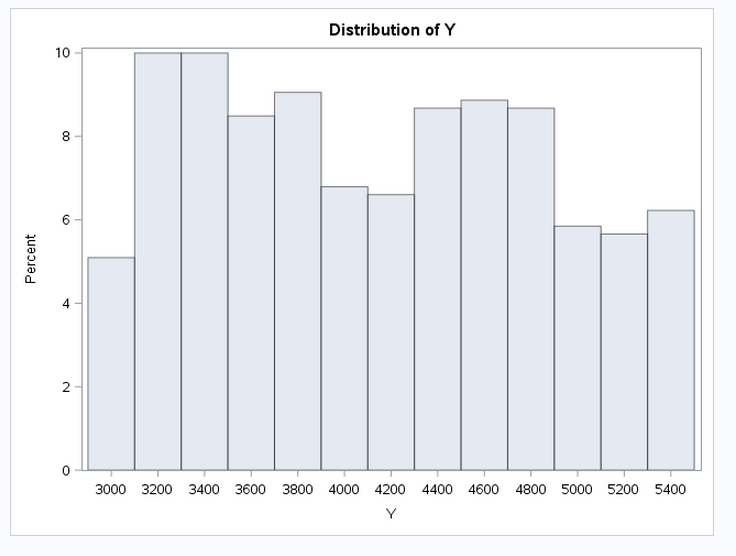
\includegraphics{Chapters/38now.png}
\caption{Zoomed In Histogram}
\label{fig:y_zoom}
\end{figure}

This indicates a departure from normality for our $Y$ variable, which might mean that the departure from normality could arise in the final model's residuals. For finding the regression equation, this isn't a problem, as we only require the residuals to have constant variance and mean of 0. It just makes statistical inferences on the parameters more difficult. We will consider an alternative model with Poisson and negative binomial distributed residuals in section \ref{sec:poisson}.



\begin{figure}
\centering
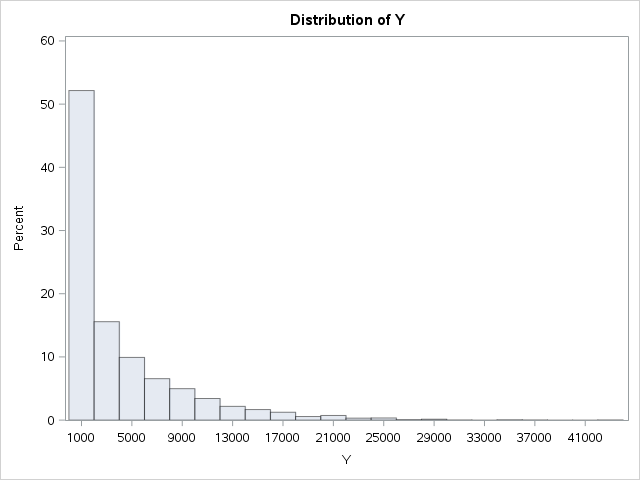
\includegraphics{Chapters/y_hist.png}
\caption{Histogram of Y}
\label{fig:y_hist}
\end{figure}




\section{Initial Regression Model}

First we check for multicollinearity within the model. Since we are going to use uncentered interaction terms in the final model, the variance inflation factor will be misleading, since most of the variables would show up as having a high VIF even when they are not collinear. Instead, I ran a model with $Y$ and only first order terms. The VIF table is in figure \ref{fig:vif}

\begin{figure}
\centering
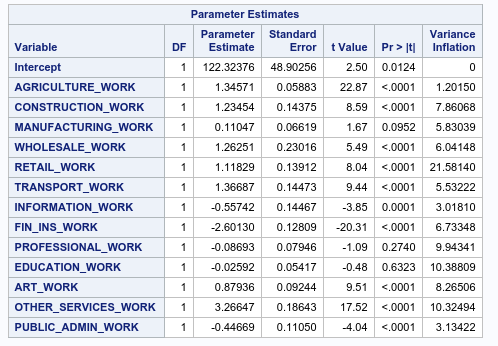
\includegraphics{Chapters/collinear.png}
\caption{VIF Table}
\label{fig:vif}
\end{figure}

Using the decision rule of $VIF>10$, we can see that retail work, educational services work, and other work have a high VIF. Other services work is the only variable of the three to have an unclear interpretation in our theoretical model, so we drop it from the regression, and run another VIF model. In the next model, education and retail services work still come up with a $VIF > 10$. Retail services is important for our conceptual model, but after running the correlation matrix, I can see that it is highly correlated with almost every other variable, which implies that retail work increases in a zip code as other work increases in those zip codes. For this reason, I've dropped it from the final model. Population size was also kept in the model since it normalizes the interpretation of the $\beta_i$s throughout the model. 

So now we run the inital regression model. The results are given in figure \ref{fig:reg}

\begin{figure}
\centering
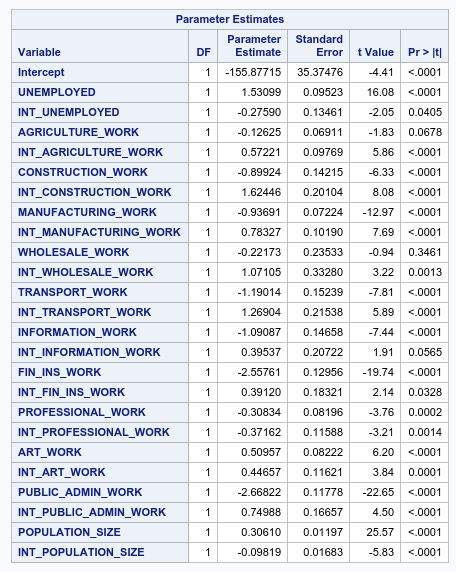
\includegraphics{Chapters/reg.png}
\caption{Initial Regression Results}
\label{fig:reg}
\end{figure}

We can see that at the $\alpha=5\%$ level, Agriculture work, Wholesale work, and the interaction term for information work are not statistically significant. We'll run two supervised model selection procedures to see what they say.

Both Akaike's information criterion and Mallow's CP criterion direct us to choose the model with all explanatory variables in it. Akaike's information criterion is minimized at 25 parameters with $AIC_p = 51610$. Mallow's CP Criterion equals 25 at 25 parameters. 

I've given above a detailed explanation of why I included interaction terms. 


Since the statistically insignificant variables had a low p-value to begin with, I decided to keep them in the model since they don't affect the values of the coefficients much when removed, and all of them have a second order term that is statistically significant. 

\section{Residual Analysis}

Looking at the leverage and residual plots, we identify one specific outlier. The diagnostic plots are given in figure \ref{fig:resid}

\begin{figure}
\centering
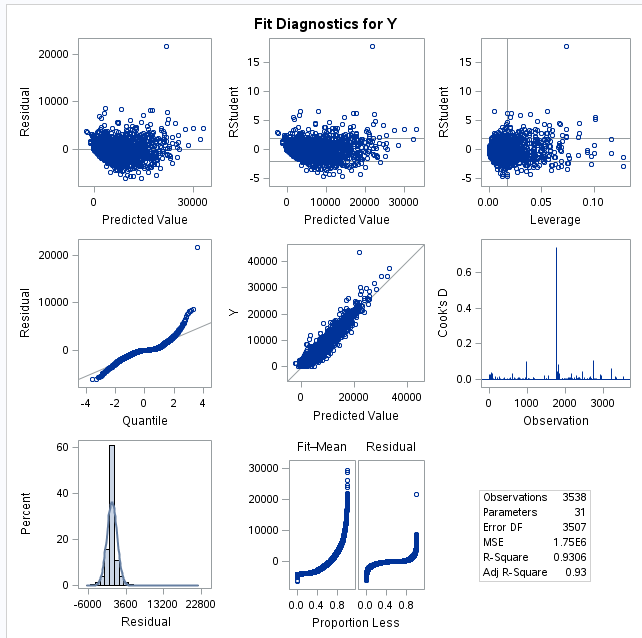
\includegraphics{Chapters/outlier.png}
\caption{Outlier Detection}
\label{fig:resid}
\end{figure}

Looking at the dataset, the point corresponds to the poverty statistic from zip code 90011. I checked a demographic database, and it looks to be correct, the zip code 90011 has a poverty level of 43.3\% compared to a statewide average of 13.8\%. Since this is not the result of a measurement error, there is not an exigent reason to delete it from the dataset. Let's run a regression without it, and see how much the values on the coefficients change. 


\begin{figure}
\centering
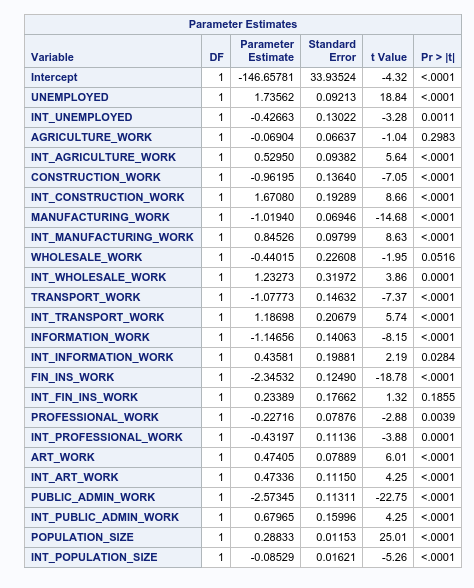
\includegraphics{Chapters/final_model.png}
\caption{Final Model OLS}
\label{fig:final_model}
\end{figure}

The coefficient values are included in \ref{fig:final_model}. It looks like the data for zip code 90011 was influential on the model for the other data. For instance, the coefficient for unemployed changed from 1.53 to 1.73. I thus delete the observation for 90011 for being an influential outlier in both the $X$ and $Y$ directions. I've also deleted its interaction term. 

Let's look at the plots of the error terms for this new model, given in figure \ref{fig:new_resid}. 

\begin{figure}
\centering
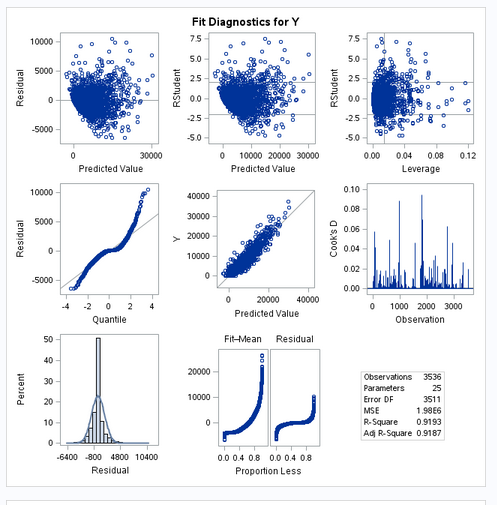
\includegraphics{Chapters/new_resid.png} 
\caption{New Residuals}
\label{fig:new_resid}
\end{figure}


The population looks to exhibit homoskedasticity by inspecting the residual versus fitted value plot to see if there is any spread. It's probably a good sign that I wouldn't even know where to set a point for a Brown Forsythe test (but I understand that is the test I would use to test it). Trivially, the mean of the residuals looks to be 0. 

Inspection of the quantile quantile plot reveals that the error terms seem to have heavy tails, which implies that the error terms might not be normally distributed. Again, the only part of our model this affects is that OLS might not be the best linear unbiased estimator for the $\beta_i$s. 

\subsection{Interpretation of Coefficients}

So now comes the fun part of the regression model. What do the terms actually mean? Since we set up the equation such that the sum of $\beta_i$ for a predictor and its interaction term make theoretical sense, the coefficient on $\beta_i$ is the expected change in the number of citizens living below the poverty level for each change in the job class $i$. The interaction term for $\beta_i$ is the number of people in addition to $\beta_i$ that we can expect to be living below the 200\% poverty level for each change in job class i.

Let's consider a concrete example. $\beta_i$ for unemployment is 1.53, and the interaction term's $\beta$ is -0.27. In a given zip code, for each additional unemployed person, you can expect 1.53 more people living below the poverty threshold (or, each 2 unemployed people correspond to 3 people living below the poverty level). However, for each additional unemployed person, you can expect only $1.53-0.27=\boxed{1.26}$ people living between 100\% and 200\% of the federal poverty level. Unemployment has a more pronounced effect on the number of people living below the poverty level than it does on the number of people living just above the federal poverty level.

For our research aims of identifying the populations that are potentially newly eligible for SNAP benefits, we want to look at variables that have a relatively large value for their interaction term. The three largest job classes are transportation, wholesale, and construction work. This is a change from the three largest poverty-prediction job classes: unemployment, art work, and the population size. It shows that the demographics change in the newly eligible SNAP beneficiaries, and presents an opportunity for changing the model of identifying new beneficiaries. 


\section{Other Regression Models}

The one remaining problem is the distribution of the residual terms. The residuals from the OLS estimate were only approximately normal, and with over 3000 observations, the central limit theorem should have brought the error terms close to normally distributed if the underlying distribution was originally anywhere close to normal. This is especially poignant when noticing that the tails of the distribution are not normal. In the central limit theorem, the rate of convergence is quickest for values closer to the population mean, and on the order of O(n) for the tails of the distribution. Thus, we should wonder if we can replace the normal assumption with an assumption that more closely matches our dataset. 


\subsection{Poisson Regression}
\label{sec:poisson}

Poisson regression is a generalized linear regression model where the errors are assumed to have a poisson distribution. The three assumptions of the Poisson regression model are:

\begin{enumerate}
\item Independence: Each observation is independently distributed
\item Homogeneity: Each observation has an error term with the same mean
\item Time Period: the measurement period is fixed
\end{enumerate}

One limitation of the Poission regression model is item number 2. In the Poisson distribution, we have that 

\[E[Y} = E[Y^2] = \lambda\]

which is a strong assumption. There is another model called Negative Binomial regression that generalizes the distribution requirement. Recall that the Negative Binomial distribution is a random variable $N$ such that
\[N \sim Pois(\lambda\]

Where 
\[\lambda \sim \Gamma[ k,\theta]\]

This lets one fit a model to a distribution with a scale and a shape parameter, then a Poisson re-distribution based on the random variable. The general rule of thumb is to run a Poisson regression first, and then run a Negative Binomial model if the dispersion value is greater than 1. The dispersion value for a Poisson regression is defined as:

\[ D = \sum_{i=1}^n \left[Y_i\log(Y_i\mu_i) - (Y_i - \mu_i)\right]\]

http://thestatsgeek.com/2014/04/26/deviance-goodness-of-fit-test-for-poisson-regression/

Put another way, it is the deviance of the model divided by its degrees of freedom. 

In our data set, we observed that assumptions one and two are held. Assumption three is also true because we are measuring the number of people in a given year and location, which is fixed. 

Most Poisson regresson models also include a link function that transforms the $Y$ data for the regression fitting, and then transforms the $X$ and $\beta$ data for the final analysis. The most common link function is $\log(Y)$, which means that the final model is:

\begin{align}
Y_i &= \exp(\beta_0+\sum_{i=1}^{p-1} \beta_i X_i\\
&= \exp(\beta_0\prod_{i=1}^{p-1}\exp(\beta_i X_i)
\end{align}

This is the link function we will be using in our regression model. We estimate $\lambda$ by the maximum likelihood estimate. Put in math, we assume that 

\begin{equation}
Y_i \sim Pois(\lambda(X_1,\cdots,X_{p-1})
\end{equation} 
Where 
\begin{equation}
\lambda(X_1,\cdots\X_{p-1}) = \exp(\beta_0 + \beta_1X_1 + \cdots \beta_{p-1}X_{p-1})) \label{eqn:realbig}
\end{equation}

The likelihood function of $X,Y$ is given as:


\begin{equation}L(\vec{\beta}) = \prod_{i=1}^{n} \frac{e^{-\lambda(\vec{X}i)}\lambda(\vec{X})^{Yi}}{Y_i!}
\end{equation}

The partial differential equation of the $l = \log(L)$ function would be a system of equations of $p$ equations in $p$ unknowns. Unfortunately, the solution is not analytic, and numerical methods must be used to obtain the solution. 


http://www.stats.uwo.ca/faculty/braun/ss3859/chapters/chapter_12/ch12.pdf

One thing to note is that on our dataset, the numbers in the population are very large, so expressions like \ref{eqn:realbig} are sensitive to very small increments in $\beta_i$. While the original model converges, it provides $\beta$ values on the order of 0.0001. For the model, we used a scaled version of the $X$ dataset:
\begin{equation}
X_s = \frac{1}{1000}X
\end{equation}

The results are given in figure \ref{fig:poisson}. Notice that the scale parameter is greater than 1, so a negative binomial regression model might probably be more appropriate. I'm not going to go into detail on that because I'm at 14 pages already, and this isn't supposed to be a book. It suffices to say that it didn't really help much in the regression.

\begin{figure}
\centering
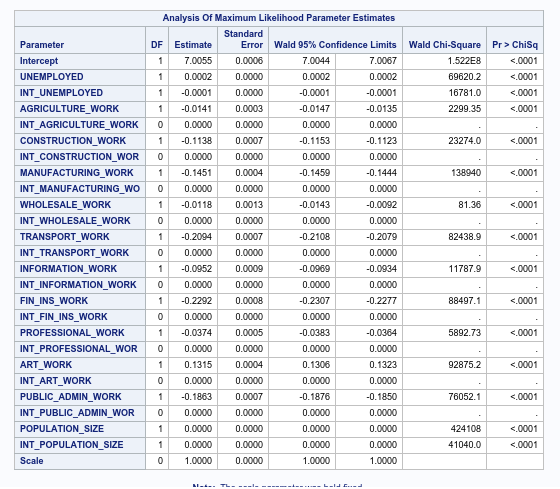
\includegraphics{poisson.png}
\caption{Poisson Regression}
\label{fig:poisson}
\end{figure}


\section{Model Testing}

So now is the fun part. Which model is better? Is it the linear regression model, or the Poisson regression model? Let's find out.

In order to test the effectiveness of the two models, we are going to divide the dataset into a training and testing dataset randomly. We will run a prediction of the $\hat{Y}$ on the testing dataset with the Poisson and linear regression models, and then compute the mean square prediction residuals from each model. The one with the lower MSPR will win the first test.

The second test will be based on the datapoints in the testing set that correspond to populations between 100\% and 200\% of the federal poverty limit, since this is the initial problem we started with. We will them compute the top 25 zip codes in terms of expected $Y$ values, and whichever model has the highest total actual $Y$ values will win the second test.

Let's do this now. The final results of our tests are given in table \ref{tab:results}.

So it looks like Ordinary least squares is the ultimate winner for our modeling of poverty levels within the zip codes of Southern California.  The MSPR of 263,815 in the testing set also matches pretty closely to the MSE in the training set of 212,000. I am pretty confident on the power of this model to predict poverty levels in Southern California, and thus the interpretation of the trends in the coefficients for planning future outreach in the SNAP benefits program.  I've selected five random results from OLS and presented them in table \ref{tab:random_five}. The results match up pretty well. 

\begin{table}[]
\centering
\begin{tabular}{c|c|c}
$n$ & $Y$ & $\hat{Y}$ & $Y -\hat{Y}$\\
\hline
1 &	7365&	9442.619305&	-2077.619305\\
2&	15477&	12942.442864&	2534.5571364\\ 
3&	332&	278.26684201&	53.733157993\\ 
4&	9852&	10914.19681&	-1062.19681\\ 
5&	22844&	19724.569354&	3119.430646 \\
\end{tabular}
\caption{Random 5}
\label{tab:random_five}
\end{table}


\begin{table}[]
\centering
\begin{tabular}{l|c|c}
Model & MSPR & Top 25 Sum  \\
\hline
Poisson & 10620589 & 226460 \\
OLS & 2247737 & 263815 \\
\hline
Winner & OLS & OLS
\end{tabular}
\caption{OLS VS Poisson}
\label{tab:results}
\end{table}

\section{Conclusion}

In this paper, we presented a use of interaction terms to decifer the differential effect that job count demographics have on two different populations with respect to income level. We found several job types to be highly correlated with the general population size, and with the remaining variables produced a model with an $R^2$ value of $92.5\%$. we then developed a Poisson regression model and tested it against the OLS model, ultimately deciding to keep the original model. Future research could investigate the effects of the zero population models on the efficacy of the count regression, particularly a zero inflated model, and identifying variables that could be used to predict the zeroes. Also we could use different count models, such as Negative Binomial regression.

This class has been a blast. 

\begin{figure}
\centering
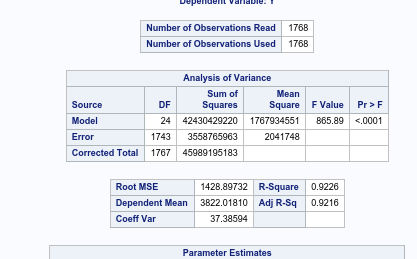
\includegraphics{Chapters/anova.png}
\caption{Anova Table}
\label{fig:my_label}
\end{figure}
\newpage

\section{References}

Cameron, A. C. and Trivedi, P. K. (2013). Regression Analysis of Count Data, 2nd Edition. Cambridge: Cambridge University Press. A comprehensive discussion of Poisson regression, with extensions to negative binomial and related models.

http://www2.sas.com/proceedings/sugi22/STATS/PAPER267.PDF

http://www2.sas.com/proceedings/sugi22/STATS/PAPER267.PDF
(2015, February 4). Retrieved December 1, 2015, from https://onlinecourses.science.psu.edu/stat504/node/169

Braun, J. (2012). Chapter 12 Lecture Notes. Retrieved December 9, 2015, from http://www.stats.uwo.ca/faculty/braun/ss3859/chapters/chapter_12/ch12.pdf

Dallal, G. (2015). Poisson Regression. Retrieved December 13, 2015, from http://www.jerrydallal.com/lhsp/poisson.htm

http://www.oecd.org/dac/povertyreduction/43280288.pdf

http://www.city-data.com/zips/90011.html
